\documentclass[12pt]{report}

\usepackage[letterpaper, hmargin=0.75in, vmargin=0.75in]{geometry}

\usepackage{
    courier,
    algorithm,
    algpseudocode,
    listings,
    underscore,
    authblk,
    hyperref,
    tikz,
    tabularx,
    float,
    graphicx,
	 color
}

\lstset{basicstyle=\footnotesize\ttfamily}

\setlength{\parindent}{0pt}

\begin{document}

\title{RTX Operating System Report}

\author{
    Tyler Babaran\\
		20457511\\
    \texttt{tbabaran@uwaterloo.ca}
    \and
    Kelly McBride\\
		20479819\\
    \texttt{ke2mcbri@waterloo.ca}
    \and
    Peter Socha\\
		20484453\\
    \texttt{psocha@uwaterloo.ca}
}

\date{April 6, 2015}

\maketitle


\tableofcontents
\listofalgorithms
\listoffigures

\chapter{Introduction}

This report is a design document outlining the RTX operating system written by Tyler Babaran, Kelly McBride, and Peter Socha as part of the SE 350 course at the University of Waterloo. The OS is written for an MCB1700 board with an LPC1768 microcontroller.\\

The purpose of this report is to provide documentation on the operating system. It will outline the kernel API available to anyone programming processes for the OS. The provided system and user processes are described in detail. Information on initialization and interrupts it also included. Finally, there is a section describing the time performance of the some of the key kernel primitives.\\

The ruling concept of the RTX detailed here is simplicity. Some of the methods used
to achieve `simplicity' are unconventional, but the idea of simplicity still holds
true. The priority queues are implemented as sorted linked lists where high priority
processes are placed first, the memory heap is implemented in a way that might 
take a few explanations, and the message-envelope structure may seem unconventional,
but each part is simple enough and they are separate concerns so that when the RTX
functions, every part functions together as a whole in a simple and expected way.

\chapter{Design Description}

\section{Global Variables and Structures}

The global variables are structures used in the RTX are primarily for initialization, though
some are core to its functionality.
\begin{itemize}
	\item \texttt{gp\_stack}: points to the last allocated stack address, used when allocating process stacks
	\item \texttt{g\_test\_procs}: an array of \texttt{PROC\_INIT} structs, used for initializing user processes
	\item \texttt{g\_proc\_table}: an array of \texttt{PROC\_INIT} structs, containing both system and user processes for initialization
	\item \texttt{gp\_pcbs}: the array containing the PCB for every process, used during context switches constantly
	\item \texttt{gp\_current\_process}: a pointer to the current process' PCB, also used constantly
	\item Process Queues: \texttt{g\_ready\_queue, g\_blocked\_on\_memory\_queue, g_blocked_on_receive_queue},
		the three process queues are global and used constantly as well, to place each process
		onto the correct queue based on its outstanding requests and messages.
\end{itemize}
In terms of global structures, both \texttt{heap\_blk} and \texttt{pcb} are global
and widely used, \texttt{heap\_blk} for allocating memory blocks in the heap, and
\texttt{pcb} for the process control blocks. Both are detailed further on.
There are also some global variables used only for the i-processes.
\begin{itemize}
	\item \texttt{g\_buffer[]}: a buffer to hold text being output
	\item \texttt{*gp\_buffer}: a pointer to \texttt{g\_buffer} so that it can be easily modified within a function
	\item \texttt{g\_char\_in}: a variable to hold one character at a time from the UART
	\item \texttt{g\_char\_out}: a variable to hold one character at a time for output to the CRT
	\item \texttt{g\_input\_buffer[BUFFER\_SIZE]}: a character array to hold user input
	\item \texttt{g\_ouptut\_buffer[BUFFER\_SIZE]}:
	\item \texttt{g\_input\_buffer\_index}: an integer to iterate through \texttt{g\_input\_buffer}
	\item \texttt{g\_output\_buffer\_index}: an integer to iterate through \texttt{g\_output\_buffer}
	\item \texttt{g\_msg\_uart}: a \texttt{msgbuf} the UART i-process uses to process input
	\item \texttt{g\_timer\_count}: increments with each clock cycle
	\item \texttt{g\_timer\_flag}: toggles to 1 when a message is sent, and back to 0 when the timer interrupt is fired
\end{itemize}

\section{Memory Management}

\subsection{Memory Structure}

The `heap' that the processes request memory blocks from is maintained as a linked list. The length of the heap is exactly enough space for thirty memory blocks of size 0x80 (128 bytes).\\

Free space nodes keep track of the length of free space following this address and a pointer to the next chunk of unclaimed blocks. These headers are written directly into the blocks as they are returned to the heap. They are free to be overwritten, the only safe header is the starting address of the heap. The heap is shifted by four bytes to protect the last block from ever being overwritten. \\

The request and release methods maintain the optimal structure of the list, deleting and overwriting excess or useless nodes.\\

\begin{figure}
	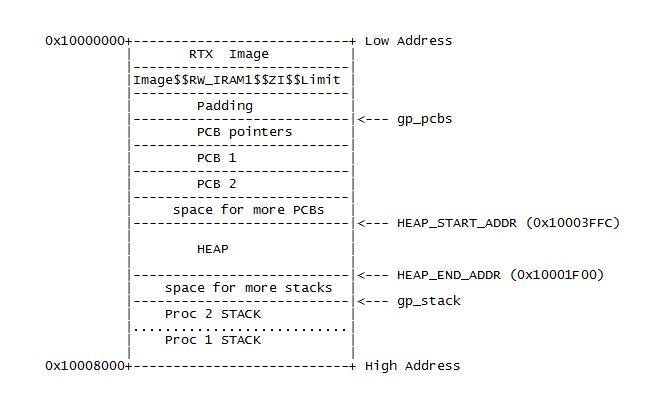
\includegraphics{memory.png}
\caption{System Memory Layout}

\end{figure}

\subsection{Requesting Memory Blocks}

\begin{minipage}{\textwidth}
\begin{lstlisting}[language=C, frame=single]
int k_request_memory_block(void);
\end{lstlisting}
\end{minipage}

First, the procedure checks if all memory blocks in the system heap have been reserved already. If so, this process becomes blocked and will be unblocked once another process releases one of the memory blocks. \\
Once a memory block is free the procedure iterates through the free space nodes like a linked list, searching for the first chunk of free space that is large enough to satisfy the request. Then the procedure passes a pointer to the first address of the block to the process and updates the heap to account for this space being reserved. \\

\begin{algorithm}
  \caption{The memory request function}
  \begin{algorithmic}[1]
    \Procedure{request\_memory\_block}{}
      \While{heap is full}
			\State {block the current process}
	  \EndWhile
	  \State {update the free space list}
	  \State {return the address of the top of the block}
    \EndProcedure
  \end{algorithmic}
\end{algorithm}

\subsection{Releasing Memory Blocks}

\begin{minipage}{\textwidth}
\begin{lstlisting}[language=C, frame=single]
int k_release_memory_block(void* memory_block);
\end{lstlisting}
\end{minipage}

Releasing memory blocks requires a pointer to a memory block. The procedure focuses on optimally returning the block to the heap list. Then it unblocks the next process waiting for a memory block, if any.

\begin{algorithm}
  \caption{The memory release function}
  \begin{algorithmic}[1]
    \Procedure{release\_memory\_block}{*memory_block}
      \If{this block is the top block of the heap}
			\State {modify heap header node (never gets overwritten)}
	  \EndIf
	  \If{there is free space immediately beneath this block}
			\State {combine them by increasing this block's length}
	  \Else { this block becomes a new block node, is added to the list}
	  \EndIf
	  \If{there is free space immediately beneath this block}
			\State {combine them by increasing this block's length}
	  \EndIf
	  \If{a process is blocked on memory}
			\State {unblock that process, release the processor}
	  \EndIf
    \EndProcedure
  \end{algorithmic}
\end{algorithm}

\pagebreak


%%%%%%%%%%%%%%%%%%%%%%%%%%%%%%%%%%%%%%%%%%%%%%%%%%%%%%%%%%%%%

\section{Processor Management}

\subsection{Process Control Structures}

The Process Control Block (PCB) is the primary process control structure. It
contains the \texttt{m_pid}, \texttt{m_priority}, and \texttt{m_state} as integers, and 
\texttt{mp_sp}, the process' stack pointer, \texttt{mp_next}, a PCB pointer used for our
process queues, and \texttt{m_queue}, the pointer to that process' message queue.
This is all of the information necessary for context switching from one process
to the next. Users cannot view nor modify any process' PCB directly.

\subsection{Process Queues}

The process queues are implemented to use one queue for all priorities, instead of a separate queue for each priority. Each {\tt PCB} contains a {\tt PCB} pointer, allowing the {\tt PCB}s themselves to be the queue nodes. \\
By using generic methods that use pointers of pointers as parameters, the same four methods are used for all process queues: \\
\begin{minipage}{\textwidth}
\begin{lstlisting}[language=C, frame=single]
void enqueue(pcb** targetQueue, pcb* element);
pcb* dequeue(pcb** targetQueue);
void remove_queue_node(pcb** targetQueue, pcb* element);
U32 is_empty(pcb* targetQueue);
\end{lstlisting}
\end{minipage}
The {\tt enqueue} method compares the priorities of each process in the queue and inserts the element beneath all processes of equal value, ensuring FIFO ordering.\\
{\tt dequeue} simply pops the highest priority element off the front of the queue.\\
The {\tt remove_queue_node} procedure is used when processes change priority and need to be removed and reinserted back into the queue. This searches the queue for a particular {\tt PCB}, based on process ID.\\
{\tt is_empty} is purely a helper function for the other three.\\

\subsection{Process Scheduling}

The scheduler is pre-emptive on I/O and inter-process communication.
The scheduling algorithm itself is very simple: take the process from the top of the ready queue. The ready queue is sorted based on priority and then by order of arrival. The null process is always the last process on the ready queue and it is chosen when there are no ready processes. The enqueuing and dequeueing procedures ensure that the processes are at the correct location, keeping both priority and order in mind. This scheduler does not use a time quantum nor pre-emption on a time quantum.\\


%%%%%%%%%%%%%%%%%%%%%%%%%%%%%%%%%%%%%%%%%%%%%%%%%%%%%%%%%%%%%

\section{Process Priority Management}

\subsection{Get Process Priority}

\begin{minipage}{\textwidth}
\begin{lstlisting}[language=C, frame=single]
int k_get_process_priority(int process_id);
\end{lstlisting}
\end{minipage}

The {\tt k\_get\_process\_priority} primitive is used to get the priority of a process. It takes a process ID as an input parameter. It outputs one of two things:\\

\begin{itemize}
\item The process's {\tt m\_priority} member if the process id is valid
\item {\tt RTX\_ERR} (equal to -1) if the process id is invalid
\end{itemize}

{\tt k\_get\_process\_priority} never modifies any process and never modifies any process queues.\\

\subsection{Set Process Priority}

\begin{minipage}{\textwidth}
\begin{lstlisting}[language=C, frame=single]
int k_set_process_priority(int process_id, int priority);
\end{lstlisting}
\end{minipage}

Process priority changing is all done through this method. After checking that the process is allowed to have its priority changed and the priority it is being set to is legal, the priority value is set and the process is removed and re-enqueued to the queue matching the process's current state. The processor is then released to allow for higher priority processes to take over.

\begin{algorithm}
  \caption{The process priority changing function}
  \begin{algorithmic}[1]
    \Procedure{set\_process\_priority}{processID, targetPriority}
		\If{processID or targetPriority are not legal}
			\State {return RTX_ERR}
		\EndIf
		\State {set processID's priority to targetPriority}
		\State {determine state}
		\State {remove queue node from its current queue}
		\State {enqueue processID's PCB into the correct queue}
    \EndProcedure
  \end{algorithmic}
\end{algorithm}

\pagebreak

%%%%%%%%%%%%%%%%%%%%%%%%%%%%%%%%%%%%%%%%%%%%%%%%%%%%%%%%%%%%%

\section{Interprocess Communication}

\subsection{Message Structure}

There are two structures used for message passing in the RTX, \texttt{msgbuf} and
\texttt{message}. \\
\begin{lstlisting}[language=C, frame=single]
typedef struct msgbuf {
	int mtype; /* user defined message type. One of message constants above  */
	char mtext[10]; /* body of the message */
} msgbuf;
\end{lstlisting}
The \texttt{msgbuf} structure is the general structure that both users and the
kernel know about. It is typically placed at the start of an allocated memory block
and contains integer \texttt{mtype} which describes the purpose of the message, be it
\texttt{KCD_REG} to register a new command type, or \texttt{DEFAULT} for a general
message, or any other of the defined types. The only other member of the \texttt{msgbuf}
structure is then \texttt{mbody}, a \texttt{char} array of size 10 to contain the 
message contents. \\
\begin{lstlisting}[language=C, frame=single]
typedef struct message {
	msgbuf* message_envelope;
	int sender_id;
	int destination_id;
	int expiry_time;
	struct message* mp_next;
} message;
\end{lstlisting}
The \texttt{message} structure is used only by the kernel and contains \texttt{message_envelope},
a pointer to the \texttt{msgbuf} within the allocated memory block, integers for the
\texttt{sender_id}, \texttt{destination_id}, \texttt{expiry_time}, and a pointer 
to another message structure \texttt{mp_next} for use in the message queues. \\
Typically the \texttt{msgbuf} structure is allocated at the start of a memory block,
and the \texttt{message} structure is allocated in the space right after, still before
the 64-byte mark.


\subsection{Sending Messages}

\begin{minipage}{\textwidth}
\begin{lstlisting}[language=C, frame=single]
int k_send_message(int process_id, void* message_envelope);
\end{lstlisting}
\end{minipage}

Message passing is implemented using a queue stucture very similar to the process queues. Processes can call this method after creating a typical {\tt message_envelope} containing a message type and a char array of the message's contents. The function call also requires a destination process that will receive this message. {\tt k\_send\_message} is the kernel primitive used to facilitate message sending.\\

The procedure begins by using {\tt message\_new} to create a {\tt message}, our kernel level wrapper for the {\tt message_envelope} containing additional necessary information such as the sender process's ID and the pointer necessary for message queue construction. The {\tt message} is then enqueued on the message queue of the destination process. If the destination process is {\tt BLOCKED\_ON\_RECEIVE}, we unblock and switch, releasing the processor to determine which process should be running next. \\

\begin{algorithm}
  \caption{The send message function}
  \begin{algorithmic}[1]
    \Procedure{send\_message}{destinationID, message envelope}
		\State {m = create message object from message envelope}
		\State {enqueue m on the destination process's message queue}
      
		\If{destination process is waiting for a message}
			\State {move destination process to READY state}
			\State {pre-empt the processor, switching to the waiting process}
		\EndIf
		\State {return RTX_OK}
    \EndProcedure
  \end{algorithmic}
\end{algorithm}

\subsection{Receiving Messages}

\begin{minipage}{\textwidth}
\begin{lstlisting}[language=C, frame=single]
int k_receive_message(int* sender_id);
\end{lstlisting}
\end{minipage}

Each process maintains its own message queue in the PCB. {\tt k\_receive\_message} is the kernel primitive used to facilitate message receiving. When a process tries to receive a message, first the procedure checks if the message queue is empty. If so, this process becomes {\tt BLOCKED\_ON\_RECEIVE} and will become unblocked by the {\tt send\_message} procedure. \\

Once a message is in the queue, the procedure dequeues the first message and returns the message envelope data containing the message type and contents. The {\tt sender\_id} pointer parameter is set as the {\tt sender\_id} from the {\tt message} wrapper for the process to cross reference and confirm this is the message it was waiting for. \\

\begin{algorithm}
  \caption{The receive message function}
  \begin{algorithmic}[1]
    \Procedure{receive\_message}{*sender_id}
      \While{message queue is empty}
			\State {block this process}
		\EndWhile
		\State {m = dequeue the top message}
		\State {set sender_id as m's sender_id}
		\State {return m's message_envelope}
    \EndProcedure
  \end{algorithmic}
\end{algorithm}

\subsection{Delayed Send}

\begin{minipage}{\textwidth}
\begin{lstlisting}[language=C, frame=single]
int k_delayed_send(int process_id, void *message_envelope, int delay);
\end{lstlisting}
\end{minipage}

The purpose of delayed sending is so that messages are not received immediately. A message will not end up in the message queue of the receiving process until after a delay period has passed. {\tt k\_delayed\_send} is the kernel primitive used to facilitate such message-passing.\\

The procedure begins by verifying its parameters, returning {\tt RTX_ERR} if any of the values are unacceptable. It then creates a {\tt message} structure using {\tt message\_new} with a delay equal to the {\tt delay} argument given. In regular message-sending, the {\tt delay} variable is set to zero. The message is finally enqueued on the message queue of the timer i-process. Regardless of the message's intended destination, it is given first to the timer i-process and all later handling is done by the timer i-process.\\

\begin{algorithm}
  \caption{The delayed send function}
  \begin{algorithmic}[1]
    \Procedure{delayed\_send}{processID, message, delay}
      \If{delay is negative}
			\State {return RTX_ERR}
		\EndIf
		\If{no process has id processID}
			\State {return RTX_ERR}
		\EndIf
		\State {m = create message object with expiry time of now + delay}
		\State {enqueue m on the timer iprocess's message queue}
		\State {return RTX_OK}
    \EndProcedure
  \end{algorithmic}
\end{algorithm}

%%%%%%%%%%%%%%%%%%%%%%%%%%%%%%%%%%%%%%%%%%%%%%%%%%%%%%%%%%%%%

\section{Interrupts and I-Processes}

\subsection{UART I-Process}

The UART i-process has two functions:

\begin{itemize}
\item Read characters entered through the keyboard
\item Output characters to the screen
\end{itemize}

The uart iprocess sometimes sends messages to the KCD and CRT processes. If this happens, a {\tt g\_uart\_flag} variable is set to 1. When the iprocess completes, the asssembly routine that handles the interrupt checks the value of {\tt g\_uart\_flag}. If the flag is true, it will call {\tt k\_release\_processor()} to give KCD and CRT a chance to immediately run.\\

\begin{algorithm}
  \caption{The uart iprocess}
  \begin{algorithmic}[1]
    \Procedure{uart_i_process}{}
		\State {g_uart_flag = 0}
		\If {receive data available}
			\State {read g\_char\_in from register}
			\If {_DEBUG_HOTKEYS is enabled}
				\State \Call{process_hot_key}{g_char_in}
			\EndIf
			\If {heap space is available}
				\State {m = \Call{k_request_memory_block}{}}
				\State {Set the mtype of m to CRT_DISP}
				\State {Set the mtext of m to g_char_in}
				\State {Send m as a message to the CRT process}
				\State {g_uart_flag = 1}
			\EndIf

			\If {g_char_in is a carriage return} 
				\If {heap space is available}
					\State {m = \Call{k_request_memory_block}{}}
					\State {Set the mtype of m to DEFAULT}
					\State {Set the mtext of m to g_input_buffer}
					\State {Send m as a message to the KCD process}
					\State {g_uart_flag = 1}
				\EndIf
				\State {reset the g_input_buffer}
			\Else
				\State {append g_char_in to g_input_buffer}
			\EndIf

		\ElsIf {output data available}
			\State {Receive the message m}
			\State {Output the mtext of m until the null terminator is reached}
			\State \Call{k_release_memory_block}{m}
		\EndIf
    \EndProcedure
  \end{algorithmic}
\end{algorithm}

The i-process's functionality requires it to request memory in order to make messages. In order to prevent the i-process from ever getting blocked, it never allocates memory if there is no free space available.\\

When the {\tt \_DEBUG\_HOTKEYS} flag is enabled, a set of characters has special status. When one of the characters below is typed, a message is printed to the screen using uart1. The messages consist of lists of processes, with the process id and priority stated line by line. These characters can be pressed at any time are not counted towards strings used for command-passing.\\

\begin{itemize}

\item {\tt !} prints the processes on the ready queue\\
\item {\tt @} prints the processes on the blocked-on-memory queue\\
\item {\tt \#} prints the processes on the blocked-on-receive queue\\
\item {\tt \$} prints the process that is currently running\\

\end{itemize}


\subsection{Timer I-Process}

The timer i-process is called by the timer interrupt handler, which runs 1000 times each second. The purpose of the iprocess is to send delayed messages and to update the global timer count {\tt g\_timer\_count}.\\

The timer i-process treats its message queue differently than the other processes in the RTX. Instead of popping messages off of its queue one at a time, it scans the entire queue each time it runs. The expiry time of each message is compared with the current time and the message is sent to the destination process if the expiry time has passed. A special non-preemptive message-sending procedure is used so that the i-process is not pre-empted before it has finished scanning the queue. This non-preemptive sender places the receiving process on the ready queue but does not run it. Instead, a flag variable {\tt g\_timer\_flag} is set that will cause {\tt k\_release\_processor()} to run when the i-process is finished (this call is not made in the process, but in the assembly wrapper that handles the interrupt).\\

The timer i-process does not use {\tt receive\_message()} to read its queue and therefore never gets blocked.\\

\begin{algorithm}
  \caption{The Timer iprocess}
  \begin{algorithmic}[1]
    \Procedure{timer_i_process}{}
		\State {disable interrupts}
		\State {increment g_timer_count}
		\State {g_timer_flag = 0}
      \For{message m in the timer iprocess's message queue}
			\If {m's expiry_time is less than the present time}
				\State {g_timer_flag = 1}
				\State {remove m from the timer iprocess's message queue}
				\State {send the message to its desintation process without preempting}
			\EndIf
		\EndFor
		\State{enable interrupts}
    \EndProcedure
  \end{algorithmic}
\end{algorithm}


%%%%%%%%%%%%%%%%%%%%%%%%%%%%%%%%%%%%%%%%%%%%%%%%%%%%%%%%%%%%

\section{System Processes}

\subsection{Null Process}

The null process has the lowest priority of any process in the operating system. It runs only when there are no ready processes to be run. When it runs, all it does is invoke {\tt k\_release\_processor()} so that the kernel can check if there is a ready process to be run.

\begin{algorithm}
  \caption{The null system process}
  \begin{algorithmic}[1]
    \Procedure{null\_process}{}
      \While{true}
			\State \Call{k_release_processor}{\null}
		\EndWhile
    \EndProcedure
  \end{algorithmic}
\end{algorithm}

\subsection{KCD Process}

The Keyboard Command Decoder process exists so that users can send console commands to the system at runtime. A command can be registered by sending the KCD process a {\tt KCD\_REG} type message. The KCD maintains a list of registered commands inside an array. When a {\tt DEFAULT} command is sent to the KCD, the KCD will try to recognize the command. If the command is found, the KCD will send a message to the process that registered the command; the message will have the {\tt KCD_DISPATCH} type. In both cases, the contents of the command are stored inside the message's {\tt mtext}. The KCD process is an intermediary between the UART i-process (which registers the keystrokes) and the eventual receiving message (which executes the command).\\

\begin{algorithm}
  \caption{The KCD System Process}
  \begin{algorithmic}[1]
    \Procedure{KCD_process}{}
      \While{true}
			\State message = \Call{receive_message}{\null}
			\If {message is of type DEFAULT}
				\State Read the mtext up to first whitespace or newline
				\State Try finding the mtext in the command array
				\If {command is found}
					\State Send KCD_DISPATCH message to the process that registered the command. Send the entire mtext as contents.
				\EndIf
			\ElsIf {message is of type KCD_REG} 
				\State Read the mtext and sending process
				\State Add the command to the command array
			\EndIf
			\State \Call{release_memory_block}{message}
		\EndWhile
    \EndProcedure
  \end{algorithmic}
\end{algorithm}

The KCD process assumes that command strings contain no whitespace. It assumes that any information between the first space and the end of the line is supplementary.\\

\subsection{CRT Process}

The CRT process is used to print text to the system console. The process waits for messages of type {\tt CRT\_DISP}. If it receives such a message, it will send it to the UART i-process and modify the {\tt IER} register so that the UART treats the message as an output message. The UART is interrupted and therefore the UART i-process will start to run immediately.\\

\begin{algorithm}
  \caption{The CRT Process}
  \begin{algorithmic}[1]
    \Procedure{crt_process}{}
      \While{true}
			\State message = \Call{receive_message}{\null}
			\If {message is of type CRT_DISPLAY}
				\State Send message to UART iprocess
				\State Set interrupt bits
			\Else
				\State \Call{release_memory_block}{message}
			\EndIf
		\EndWhile
    \EndProcedure
  \end{algorithmic}
\end{algorithm}

%%%%%%%%%%%%%%%%%%%%%%%%%%%%%%%%%%%%%%%%%%%%%%%%%%%%%%%%%%%%%

\section{User Processes}

\subsection{Wall Clock Process}

The wall clock process is used to display the time in 24-hour format. If the clock is on, it will print the time on the screen each second by sending messages to the CRT process. The process maintains second-by-second timing by sending itself delayed messages with a delay of 1000 milliseconds.\\

The wall clock process registers three commands with the KCD when it initializes. By typing commands into the console, the user can control the wall clock's behaviour. When the process launches, the wall clock starts as inactive.\\

\begin{itemize}

\item {\tt \%WR} - Sets the clock time to 00:00:00 and sets the clock to active.\\
\item {\tt \%WT} - Sets the clock to inactive. Cancels any scheduled future clock ticks.\\
\item {\tt \%WS hh:mm:ss} - Sets the clock to active with the given time in 24-hour format.\\

\end{itemize}

The wall clock process relies on memory blocks to send display messages to the CRT process and to send itself delayed messages to re-awaken itself. If system memory has been depleted, it will be unable to properly funcion.\\

\subsection{Set Priority Process}

\begin{minipage}{\textwidth}
\begin{lstlisting}[language=C, frame=single]
%C process_id new_priority
\end{lstlisting}
\end{minipage}

The {\tt set\_process\_priority()} primitive described earlier can be used to programmatically change the priority of any process that is not a system process. It is, however, a programmatic call that must be set in user code in advance. The Set Priority process allows users to change the priority of a process at runtime using the {\tt \%C} command.\\

The priority change takes effect immediately. If the user enters invalid parameters, \"Error\" will be printed to the screen and the command will be ignored.\\

\begin{algorithm}
  \caption{The Set Priority Process}
  \begin{algorithmic}[1]
    \Procedure{set_priority_proc}{}
		\State{register with KCD as \%C command}
      \While{true}
			\State message = \Call{receive_message}{\null}
			\State parse message mtext to get a process_id and new_priority
			\If {Setting process_id to new_priority is a valid operation}
				\State \Call{set_process_priority}{process_id}{new_priority}
			\Else
				\State {make and send an \"Error\" message to CRT}
			\EndIf
			\State \Call{release_memory_block}{message}
		\EndWhile
    \EndProcedure
  \end{algorithmic}
\end{algorithm}

\subsection{Stress Test Processes}

The stress test processes are a collection of three user processes called A, B, and C. The three of them are used to test how the system copes with the depletion of heap blocks in memory.\\

Process A waits until it receives a {\tt \%Z} command, after which it will repeatedly request memory, make messages, and send those messages to Process B.\\

Process B receives messages from A and sends them to Process C.\\

Process C receives messages from Process B. Every 20th message, it prints \"Process C\" to the screen by modifying B's message and passing it to the CRT. Every 20th message, it will then request a memory block and send itself a delayed {\tt WAKEUP10} message to be received in 10 seconds. During those 10 seconds, it goes into a hibernation state, receiving messages from B and putting them on its local queue, but otherwise not doing anything.\\

In general, Process A requests memory blocks and Process C ends up releasing them. If Process C's priority is too low, memory blocks may end up never being released and we may end up in deadlock.\\

\section{Initialization}

Process Initialization is comprised of four parts:
\begin{itemize}
	\item Process table setup: each process' data (\texttt{m_pid}, \texttt{m_stack_size},
		\texttt{mpf_start_pc}, \texttt{m_priority}) is entered in \texttt{g_proc_table}
		for further initialization and housekeeping.
	\item PCB intialization and stack allocation: the data from \texttt{g_proc_table}
		is used to populate the PCBs in \texttt{gp_pcbs} and each process is
		allocated a stack of size \texttt{m_stack_size}.
	\item PCB enqueueing: every PCB is enqueued in the ready queue, \texttt{g_ready_queue}.
	\item Messages to set up some processes: processes which register a \texttt{KCD}
		command often do so as their first action so that the command can be
		used as soon as possible.
\end{itemize}
Once these steps are complete, the scheduler selects the first process to run
from the ready queue and execution begins.


\section{Testing}

We used the user processes to test the functionality of our system. We implemented a dynamic test polling system, where the user processes updated a list of execution ordering as they switched between each other.\\

This list is constantly compared with a preset expected execution order, and discrepencies cause the TEST_PASSED flag to flip. Since the texts printed in order, it became easier to identify at what point in the test execution the unexpected behaviour occurred.\\

At each stage of development we used the user processes to test the limits of the system. Extensive memory block requesting, message passing, and priority switching stressed our data structures, revealing critical design flaws and bugs that would have otherwise gone overlooked. \\

Towards the end of the project, we implemented the second system timer to observe how long executions would take to execute. This allowed us to investigate inefficiencies and determine where our code base could be improved.\\

\chapter{Major Design Changes}


\section{Structure of Process Queue}

By the end of P1 we had the blocked and ready queue each use a separate set of queueing functions. The introduction of the \"blocked on receive\" queues forced us to rework the queueing methods to operate generically, passing a reference to the queue head along with each function call.\\
This cleaned and simplified a large section of the code base, greatly reducing our repeated code.\\

\section{Heap Faults}
Through stress tests we encountered a unique edge case in our memory heap assignment. The order that the KCD and Wall Clock requested blocks lead us to a chain of memory leaks that would have otherwise gone unnoticed. These leaks were caused by incorrectly calculating the shift required to protect the head heap node, causing it to be overwritten and the entire heap structure would be lost.




\chapter{Lessons Learned}

\section{Source Control and Code Management}

We used GitHub as a repository for our code, which proved to be very helpful. However, we never developed any systematic protocols for using GitHub and we did not take advantage of many of its features.\\

Nearly all development was done on the master branch and was pushed directly to the master branch. We rarely coded on the same module at the same time so conflicts were surprisingly rare. However, we did not have a systematic code review process. While this saved us time in the short run, it meant that team members did not have much of a chance to learn about the code that the other team members were writing. The team became overly specialized; many of the modules in the OS were well-understood by only one team member. A more systematic review process may have helped keep all members on the team well-grounded on all aspects of the OS.\\

\section{Team Dynamics and Scheduling}

There were no major conflicts between any of the team members, which proved beneficial for all of us.\\

We did not have a systematic process for allocation and scheduling of tasks. Usually a release cycle would begin as a free-for-all with members choosing parts they wanted to work on. Later on in the cycle, an allocation system would be determined, but it was informal, frequently did not go according to plan, and rarely carried any concrete deadlines for individual group members.\\

With P1 and P2 in particular, we encountered time trouble and needed to use a late day for each. We could have avoided this problem by allocating responsibilities more precisely and maintaining deadlines for the main milestones.\\

\chapter{Timing and Analysis}

In order to do timing, a second timer (called \"timer 1\") was programmed. Whereas timer0 interrupted once every millisecond, timer1 never interrupts and never does anything other than maintain a count. Like timer0, timer1 operated at a speed of 100MHz.\\

The timer test code was added to the user test processes, with the tests conducted in {\tt proc5()} after all the regular tests had been completed. The three primitives that had their time measured were {\tt k\_request\_memory\_block()}, {\tt k\_send\_message()}, and {\tt k\_receive\_message()}. The test was designed so that there would be no blocking or pre-emption during any of these calls. Each of these functions was called ten times inside a loop and the elapsed time was measured using the timer's {\tt TC} register. By writing certain values to the timer's {\tt TCR} register, we were able to programmatically start, stop, and reset the timer during and between tests.\\

The raw data proved to be very consistent and exhibited zero variance in 24 total runs. Since the timer ticked at 100MHz, it meant that each clock tick represented 10ns in time. Since each time value was obtained on a sample of 10 calls made consecutively, we divide by 10 to get the time elapsed per individual call. Here is the data, represented as ns per call.\\

\begin{figure}[H]

\begin{tabular}{| c | c | c | c | }
    \hline
     & {\tt k\_request\_memory\_block} & {\tt k\_send\_message} & {\tt k\_receive\_message}\\
    \hline
    Time (ns) & 420 & 1028 & 866\\
    \hline
\end{tabular}

\caption{Timing Test Results}

\end{figure}

Judging by the high consistency of the results, the hardware always executed the code in the same predictable manner without any optimizations or stalls.\\

The primitives for message-handling are more expensive than the primitive for memory. This difference is likely due to the fact that the message primitives work with the {\tt message} object type, which is larger and more complex than the {\tt heap\_blk} object type used to manage heap blocks.\\

\end{document}
